\documentclass{article}
\usepackage{graphicx}
\usepackage[margin=1.5cm]{geometry}
\usepackage{amsmath}

\begin{document}

\title{Tuesday Reading Assessment: Unit 0, Coulomb's Law and E-fields}
\author{Prof. Jordan C. Hanson}

\maketitle

\section{Memory Bank}

\begin{itemize}
\item $\vec{F}_{12} = k q_1 q_2 / r^2 ~~\hat{r}$ ... Coulomb force.
\item $k = 8.988 \times 10^{9}$ N C$^{-2}$ m$^{2}$ ... The constant of proportionality in Coulomb force.
\item $\vec{F} = q\vec{E}$ ... Definition of an electric field.
\item $1e = -1.602 \times 10^{-19}$ Coulombs ... Charge of an electron.
\item $1p = +1.602 \times 10^{-19}$ Coulombs ... Charge of a proton.
\end{itemize}

\section{Coulomb Force}

\begin{enumerate}
\item Suppose you have a charge of +1 nC, or $10^{-9}$ Coulombs, separated from another identical charge.  (a) What will be the force between them? (b) Will the charges accelerate toward each other or away from each other? \\ \vspace{2cm}
\begin{figure}[ht]
\centering
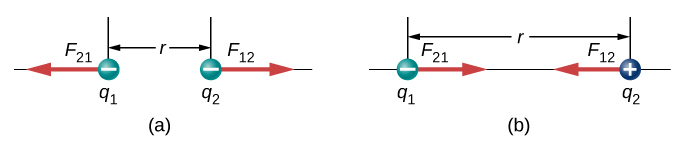
\includegraphics[width=0.7\textwidth]{Coul.png}
\caption{\label{fig:coul} With the Coulomb force, like charges repel each other, and opposite charges attract.}
\end{figure}
\item How many protons are required to create a \textit{total charge} of +1 nC, or $10^{-9}$ Coulombs? \\ \vspace{1cm}
\item If two charges are a distance $r$ apart, and then $r$ is tripled, by what factor does the force decrease?
\begin{itemize}
\item A: 3
\item B: 6
\item C: 9
\item D: 12
\end{itemize}
\end{enumerate}

\end{document}
